\documentclass[a4paper]{exam}

\usepackage{graphicx}
\usepackage{siunitx}
\DeclareSIUnit{\revolution}{rev}
\DeclareSIUnit{\rpm}{\revolution\per\minute}
\DeclareSIUnit{\lightyear}{ly}

\begin{document}
  \section*{L3 Physics: Revision questions for part 1 (Mechanics)}
  Questions 1 and 2 are from Howison, chapter 5. Questions 4, 5, 6, and 7 are from past exams (2014, 2018, 2014 and 2014, respectively).
  \begin{questions}
    \question John is a trampoline artist. He warms up by working his arms and legs until he is jumping high and vertically above
              the trampoline mat.

              On one occasion as he leaves the mat, John's total kinetic energy (both linear and rotational) is \SI{2200}{\joule}.
              At the top of the jump his linear speed is momentarily zero and he has gained \SI{1400}{\joule} of gravitational potential energy.
      \begin{parts}
        \part At the top of the jump, assuming mechanical energy is conserved, calculate (i) John's height above the mat, and (ii) John's
              rotational kinetic energy.
        \part At the top of the jump, the angular speed of John's sumersault is \SI{18}{\radian\per\second}. Calculate John's rotational
              inertia about his centre of mass.
        \part To complete the sumersault while in the air, John folds his body into a tucked position, causing it to rotate at a faster
              rate. At the end of the rotation he straightens his body and lands back on the mat in an upright position. Explain why this
              tucking causes John's body to rotate faster than if he remains in the untucked position.
      \end{parts}
    \question A solid, uniform disc rolls from rest down a ramp of height $ h $. At the bottom of
              the ramp the disc has translational speed $ v $. Show that $ v = \sqrt{\frac{4}{3}gh} $.

    \question A space station is shaped like a long, hollow cylinder spinning around its long axis. The radius
              of the cylinder is \SI{1}{\kilo\metre}, and the cylinder is rotating with an angular speed $ \omega $.
              How large must $ \omega $ be for a person standing on the inside of the cylinder to feel a centripetal
              acceleration equal to the usual pull of gravity (\SI{9.81}{\metre\per\second})?
    \question The mass of Mercury is \SI{3.30e23}{\kilo\gram}. Mercury has a period of rotation of \SI{5.067e6}{\second}.
              Show that a satellite needs to be positioned \SI{2.43e8}{\metre} from the centre of Mercury so that it
              remains stationary from the point-of-view of an observer on that planet.
    \question
      \begin{parts}
        \part A spring of length $L$ and spring constant $k$ is cut into two parts of lengths $ L_1 $ and $ L_2 $ with
              spring constants of $ k_1 $ and $ k_2 $ respectively. Show that
              \begin{displaymath}
                \frac{1}{k} = \frac{1}{k_1} + \frac{1}{k_2}.
              \end{displaymath}
        \part Consider the situation shown below with two springs of spring constants $ k_1 $ and $ k_2 $ connected together and linking masses
              $ m_1 $ and $ m_2 $, which sit on a frictionless surface. The equilibrium lengths of the springs are $ L_1 $ and $ L_2 $, respectively,
              and the centre of mass of $ m_1 $ lies at $ x_1 $ and the centre of mass of $ x_2 $ lies at $ x_2 $.

              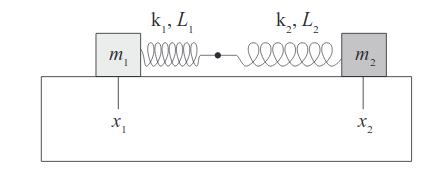
\includegraphics[width=0.4\textwidth]{springs-nzqa2018}

              Mass $ m_1 $ is held fixed while a force $ F_0 $ is applied to mass $ m_2 $ in the direction of mass $ m_1 $.
              Using the result of part (a), show that the change in position of mass $ m_2 $ is
              \begin{displaymath}
                \Delta x_2 = F_0 \frac{k_1 + k_2}{k_1 k_2}.
              \end{displaymath}
        \part Both masses are now released simultaneously. The values for the masses and spring constants are
              $ m_1 = \SI{2.0}{\kilo\gram} $, $ m_2 = \SI{3.0}{\kilo\gram} $, $ k_1 = \SI{5.0}{\newton\per\metre} $,
              and $ k_2 = \SI{10}{\newton\per\metre} $, and the force $ F_0 = \SI{2.0}{\newton} $. Assume the mass
              of the springs is negligible compared to $ m_1 $ and $ m_2 $.

              Describe in detail the resulting motion of the two masses.
        \part Show that the maximum velocity reached by mass $ m_2 $ is \SI{0.40}{\metre\per\second}.
        \part Explain how the motion of the system would be altered if the mass of the springs was not negligible compared to $ m_1 $ and $ m_2 $.
      \end{parts}
    \question A vertical pendulum is set up, hanging from a ceiling. The length of the cord (of negligible mass) is \SI{1.55}{\metre}. The bob
              has a mass of \SI{1.80}{\kilo\gram}.
      \begin{parts}
        \part Calculate the length of time it takes for the bob to swing from one side to the other.
        \part Explain how the forces acting on the bob change the bob’s speed as it travels from the point of
              release to the centre.
        \part The bob is released again in such a way that it swings in a horizontal circular path, with radius \SI{0.290}{\metre}, as a conical pendulum.
          \begin{subparts}
            \subpart By first calculating the size of the angle that the cord makes with the vertical, show that the tension
                     force in the cord is \SI{18.0}{\newton}.
            \subpart Calculate the speed that the mass must have been given when released, in order to attain
                     a horizontal circular path at a radius of \SI{0.290}{\metre}.
          \end{subparts}
      \end{parts}
    \question A system consists of two discs, A and B, attached together with a light cord. The discs slide across
              a frictionless surface. Disc A has mass \SI{0.517}{\kilo\gram} and disc B has mass \SI{0.684}{\kilo\gram}. Disc B is stationary,
              and disc A is moving towards disc B with a speed of \SI{1.21}{\metre\per\second}.
      \begin{parts}
        \part Show that the speed of the centre of mass of the system is \SI{0.521}{\metre\per\second}.
        \part The discs collide and after the collision they are moving at right angles to each other. Disc A receives an impulse of \SI{0.250}{\newton\second}.
          \begin{subparts}
            \subpart Show that the speed of disc B after the collision is \SI{0.365}{\metre\per\second}.
            \subpart Determine the size of the momentum of disc A after the collision.
          \end{subparts}
        \part The discs continue to slide until the cord is fully extended. When this happens, both discs change their speed and direction.
              By considering the force(s) that act on the discs, explain why the momentum of the system must be conserved.
      \end{parts}
    \question What is the escape velocity of a human from Earth? State any assumptions you make.
  \end{questions}

\vspace*{\fill}
This version: \today

\end{document}
